\documentclass[aspectratio=169]{beamer}
%\documentclass[aspectratio=43]{beamer}

\usepackage{graphicx}  % Required for including images
\usepackage{natbib}
\usepackage{booktabs} % Top and bottom rules for tables
\usepackage{amssymb,amsthm,amsmath}
\usepackage{exscale}
\usepackage{natbib}
\usepackage{tikz}
\usepackage{listings}
\usepackage{color}
\usepackage{animate}
\usepackage{bm}
\usepackage{etoolbox}

% Setup TikZ
\usepackage{tikz}
\usetikzlibrary{arrows}
\tikzstyle{block}=[draw opacity=0.7,line width=1.4cm]
% Setup hyperref
\usepackage{hyperref}
\hypersetup{colorlinks=true}
\hypersetup{citecolor=porange}
\hypersetup{urlcolor=porange!80!}
\hypersetup{linkcolor=porange}

\newtheorem{proposition}{Proposition}
\newtheorem{remark}{Remark}
\newtheorem{principle}{Principle}

%% Writing quarters
\newcommand{\wQ}[1]{{\textcolor{white}{Q#1}}}
\newcommand{\bQ}[1]{{Q#1}}

% Uncomment appropriate command to disable/enable hiding
%\newcommand{\mypause}{\pause}
\newcommand{\mypause}{}
\newcommand{\myb}[1]{{\color{blue} {#1}}}

%% Commonly used macros
\newcommand{\eqr}[1]{Eq.\thinspace(#1)}
\newcommand{\pfrac}[2]{\frac{\partial #1}{\partial #2}}
\newcommand{\pfracc}[2]{\frac{\partial^2 #1}{\partial #2^2}}
\newcommand{\pfraca}[1]{\frac{\partial}{\partial #1}}
\newcommand{\pfracb}[2]{\partial #1/\partial #2}
\newcommand{\pfracbb}[2]{\partial^2 #1/\partial #2^2}
\newcommand{\spfrac}[2]{{\partial_{#1}} {#2}}
\newcommand{\mvec}[1]{\mathbf{#1}}
\newcommand{\gvec}[1]{\boldsymbol{#1}}
\newcommand{\script}[1]{\mathpzc{#1}}
\newcommand{\eep}{\mvec{e}_\phi}
\newcommand{\eer}{\mvec{e}_r}
\newcommand{\eez}{\mvec{e}_z}
\newcommand{\iprod}[2]{\langle{#1}\rangle_{#2}}

\DeclareMathAlphabet{\mathpzc}{OT1}{pzc}{m}{it}

%% Autoscaled figures
\newcommand{\incfig}{\centering\includegraphics}
\setkeys{Gin}{width=0.9\linewidth,keepaspectratio}

%Make the items smaller
\newcommand{\cramplist}{
	\setlength{\itemsep}{0in}
	\setlength{\partopsep}{0in}
	\setlength{\topsep}{0in}}
\newcommand{\cramp}{\setlength{\parskip}{.5\parskip}}
\newcommand{\zapspace}{\topsep=0pt\partopsep=0pt\itemsep=0pt\parskip=0pt}

\newcommand{\backupbegin}{
   \newcounter{finalframe}
   \setcounter{finalframe}{\value{framenumber}}
}
\newcommand{\backupend}{
   \setcounter{framenumber}{\value{finalframe}}
}

\usetheme[bullet=circle,% Use circles instead of squares for bullets.
          titleline=true,% Show a line below the frame title.
          ]{Princeton}

\title[{\tt }]{Discontinuous Galerkin Schemes}%
\author[https://ast560.rtfd.io]%
{Ammar H. Hakim ({\tt ammar@princeton.edu}) \inst{1}}%

\institute[PPPL]
{ \inst{1} Princeton Plasma Physics Laboratory, Princeton, NJ %
}

\date[3/30/2021]{Princeton University, Course AST560, Spring 2021}

\begin{document}

\begin{frame}[plain]
  \titlepage
\end{frame}

\begin{frame}{Nonlinear flux limiters: Getting around Godunov's Theorem}
  To get around Godunov's Theorem we need to construct a
  \emph{nonlinear scheme}, even for linear equations. One apporach is
  to use nonlinear flux-limiters:
  \begin{align*}
    \mvec{F}_{j+1/2} = \phi(r_{j+1}) \mvec{F}^H_{j+1/2} + \big(1-\phi(r_{j+1})\big) \mvec{F}^L_{j+1/2}
  \end{align*}
  where $\phi(r)>0$ is a \emph{limiter} function: chooses between
  \emph{high-order} and \emph{low-order} flux.
  \begin{itemize} 
  \item What are the low- and high-order fluxes? For high-order
    fluxes: use either symmetric or upwind-biased recovery to
    construct the flux. For low-order use first-order upwind-biased
    fluxes.
  \end{itemize}
\end{frame}

\begin{frame}{Nonlinear flux limiters}
  \small
  \begin{columns}
    \begin{column}{0.5\linewidth}
      The limiter function $\phi(r)$ depends on an estimate of the
      \emph{relative} slopes in cell. For example, one choice is
      \begin{align*}
        r_{j+1/2} = \frac{\textrm{\textrm{slope at upwind-edge}}}{\textrm{slope at } j+1/2}
      \end{align*}
      (For systems of equations one needs limit each eigenvector
      instead). With this, choose a function that maintains
      \emph{total-variation diminishing} (TVD) property. Eg, min-mod
      limiter
      \begin{align*}
        \phi(r) = \max\big(0, \min(2r, (1+r)/2,2) \big).
      \end{align*}
    \end{column}
    
    \begin{column}{0.5\linewidth}
      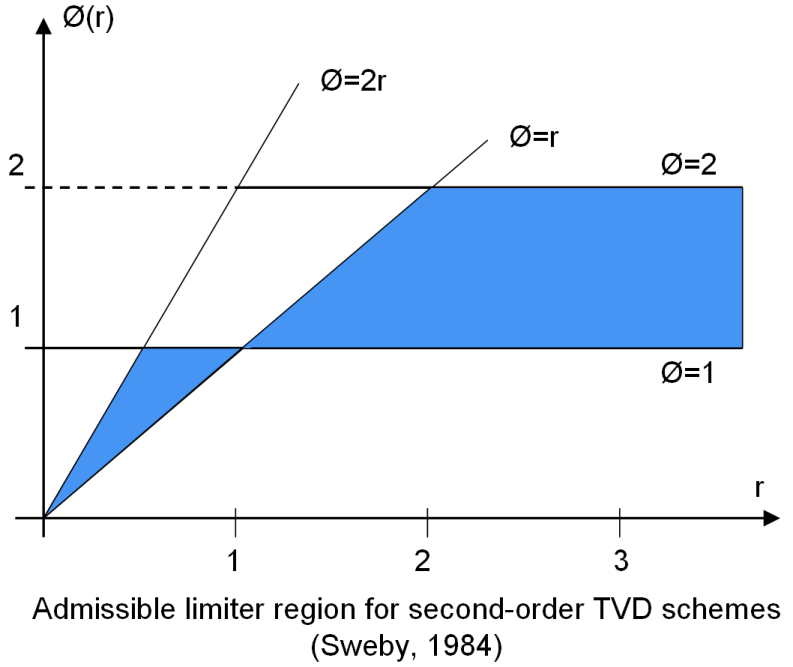
\includegraphics[width=\linewidth]{LimiterRegion.png}
    \end{column}
  \end{columns}
  See Wikipedia page
  \url{https://en.wikipedia.org/wiki/Flux_limiter}. (Not very
  high-quality but gives you a general idea).
\end{frame}

\begin{frame}{Nonlinear flux limiters: No ``Perfect'' Limiter!}
  \small
  \begin{columns}
    \begin{column}{0.5\linewidth}
      \begin{itemize}
      \item Unfortunately, there is no perfect limiter (though some
        come close to perfection): depends on problem and best to
        implement many!
      \item Most limiters ``chop off'' genuine maxima/minima: notice
        that $\phi(r<0) = 0$ which means that if there is a genuine
        maxima/minima then low-order flux is selected.
      \item Tricky to distinguish step-function from parabola!
        ``Best'' limiter (IMO): Suresh and Huynh, JCP {\bf 136}, 83-99
        (1997). Not an easy paper to understand.
      \end{itemize}
    \end{column}
    
    \begin{column}{0.5\linewidth}
      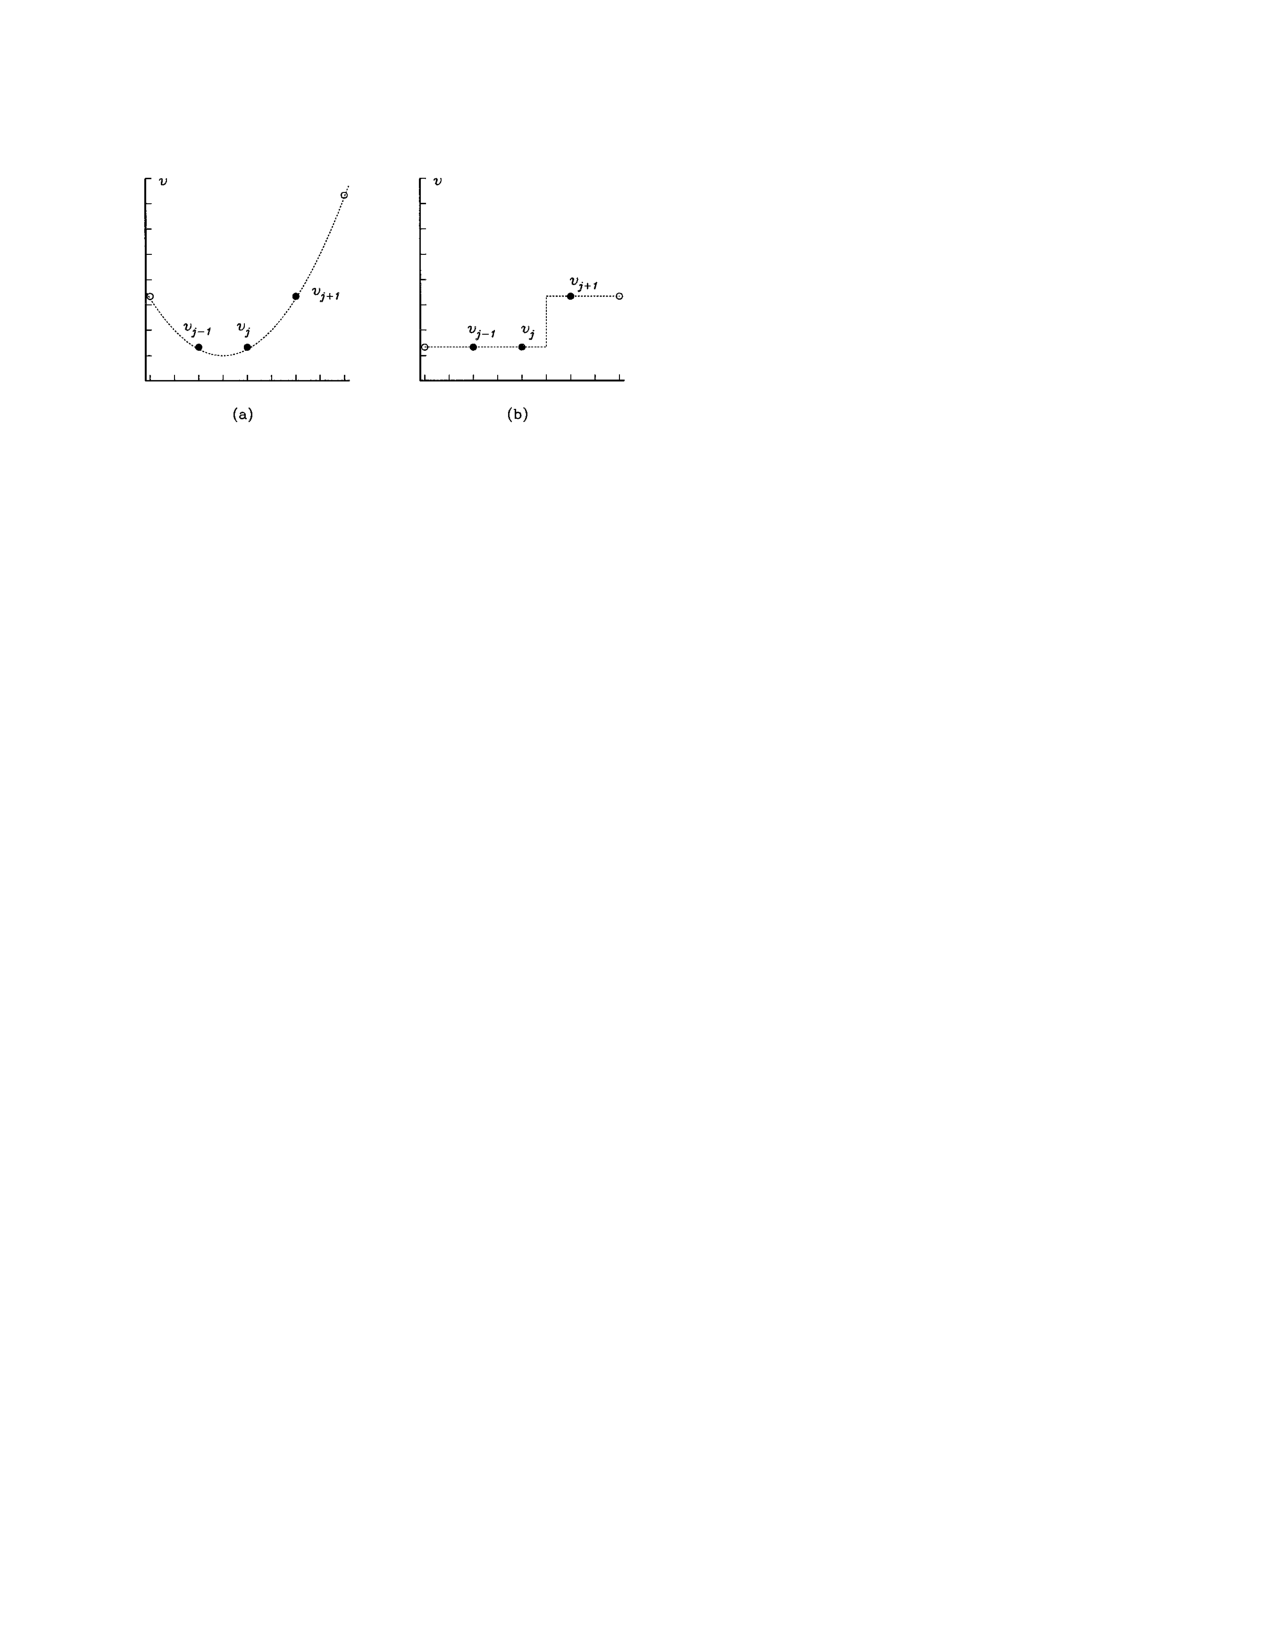
\includegraphics[width=\linewidth]{suresh-huynh.pdf}
    \end{column}
  \end{columns}
\end{frame}  

\begin{frame}{Generalizing recovery: path to discontinous Galerkin schemes}
  \begin{itemize}
  \item In FV scheme we used \emph{cell-averages} to recover interface
    values for use in numerical fluxes%
    \mypause%
  \item What if we store more than just cell-averages? One can imagine
    in addition, mean-slope, mean-quadratic moments. Lead naturally to
    the concept of discontinous Galerkin schemes.
  \end{itemize}
  \mypause%
  The key connection is the concept of \emph{weak-equality}. Consider
  an interval $I$ and select a finite-dimensional function space on
  it, spanned by set of basis functions $\{ \psi_k \}$,
  $k=1,\ldots,N$. Choose an inner product, for example
  \begin{align*}
    (f, g) \equiv \int_I f(x) g(x) \thinspace dx.
  \end{align*}  
\end{frame}

\begin{frame}{Weak-equality}
  \small
  \begin{definition}[Weak equality]
    Two functions, $f$ and $g$ are said to be \emph{weakly equal} if
    \begin{align*}
      (\psi_k,f-g) = 0
    \end{align*}
    for all $k=1,\ldots,N$. We denote weak equality by
    \begin{align*}
      f \doteq g.
    \end{align*}
  \end{definition}  
  \begin{itemize}
  \item When we recovered polynomials across an interface in FV scheme
    we effectively choose a function space, $\{1 \}$ , with only
    \emph{one} basis function!
  \item In DG we can choose as many as we like: allows significant
    flexibility in designing accurate and compact schemes; suprisingly
    accurate for some problems.
  \end{itemize}
\end{frame}
  
\end{document}


\begin{frame}{}
\end{frame}

\begin{columns}
  
  \begin{column}{0.6\linewidth}
  \end{column}
  
  \begin{column}{0.4\linewidth}
    \includegraphics[width=\linewidth]{fig/Kinsey_2011_Pfus_vs_T.pdf}
  \end{column}
\end{columns}

% ----------------------------------------------------------------
